\documentclass[12pt]{article}
%\usepackage[cp1251]{inputenc}
\usepackage[utf8]{inputenc}
\usepackage[T2A,T1]{fontenc} 
\usepackage[bulgarian]{babel}
\usepackage{amssymb,amsmath,amsfonts,amstext,amscd,latexsym}
\usepackage{graphicx}
\usepackage{amsmath}
\usepackage{amsthm}
\newtheorem*{lemma}{Лема}
\newtheorem*{theorem}{Теорема}
\newtheorem*{definition}{Дефиниция}
\usepackage[shortlabels]{enumitem}
\usepackage[colorinlistoftodos]{todonotes}
\usepackage{braket}
\usepackage{systeme}
\usepackage{hyperref}
\usepackage{titling}
\usepackage{xcolor}
\hypersetup{
	colorlinks   = true, %Colours links instead of boxes
	urlcolor     = blue, %Colour for external hyperlinks
	linkcolor    = blue, %Colour of internal links
	citecolor   = blue %Colour of citations
}
\usepackage[superscript]{cite}
\usepackage[font={small,it}]{caption}
\usepackage[geometry]{ifsym}
\usepackage{listings}
\usepackage{float}
\usepackage{color}
\usepackage{svg}

\begin{document}
	\begin{titlepage}	
		\begin{center}
		
		\newcommand{\HRule}{\rule{\linewidth}{0.5mm}} % Defines a new command for the horizontal lines, change thickness here
		
		
		\textsc{\LARGE Софийски университет }\\[0.3cm]
		\textsc{\LARGE "Св. Климент Охридски" }\\[0.3cm]
		\textsc{\Large Факултет по математика и информатика }\\[0.5cm]
		\textsc{\Large Представяне и моделиране на знания }\\[0.1cm]
		%\fontsize{size}{baselineskip}
		
		
		\vspace{15pt}\centering спец. Изкуствен интелект, I курс, летен семестър \newline учебна година 2025/2026
		\vspace{30pt}
		
		\begin{minipage}{0.4\textwidth}
			\begin{flushleft}\large
				\emph{Изготвил:} \\
				Кристиян Симов \\ 
				фак. номер 4MI3400288 \\ 
				група: 1 %Попълнете вашето име, факултетен номер и група.
			\end{flushleft}
		\end{minipage}
		~
		%\begin{flushleft}
		\begin{minipage}{0.4\textwidth}
			\begin{flushright}
				\large
				\emph{Дата:}\\
				08. 01. 2026 г. % Попълнете датата на предаване
				\\София 
			\end{flushright}
		\end{minipage}\\[1cm]
		%\end{flushleft}
		\bigskip
		{\large \textbf{Онтология на надразред динозаври}}\\
		{\large \textbf{(система от първи тип)}}\\[1cm] 
		%\includegraphics{rsz_sofia_university_logo.png}\\[1cm] 
		\includegraphics{logo_su_no_text.png}\\[1cm]
		\vfill % Fill the rest of the page with whitespace
		\end{center}
	\end{titlepage}
	
	
	\tableofcontents
	
	\newpage
	
	\section{Въведение}\label{sec:introduction}
	
	\paragraph{}
	Динозаврите (Dinosauria) са надразред животни от клас Влечуги (Sauropsida). В
	продължение на повече от 160 млн. години, започвайки от късния триас преди около 230 млн.
	години, те са най-широко разпространените сухоземни гръбначни животни на Земята. В края
	на периода креда, преди около 65 млн. години, динозаврите претърпяват катастрофално
	масово измиране, от което оцеляват само някои птици, също част от групата на динозаврите,
	обособила се през юра.
	\paragraph{}
	Динозаврите са много разнородна група животни, а птиците, с повече от 9 хил. вида са
	най-разнородната група съвременни гръбначни след бодлоперките. Освен птиците,
	палеонтолозите разграничават над 500 рода и 1000 вида динозаври. Динозаврите
	присъстват на всички континенти, както като съществуващи днес видове птици, така и
	като фосилни находки. Част от динозаврите са растителноядни, а други – хищни, някои
	се придвижват на два крака, други – на четири, а трети могат да ходят и на два, и на
	четири крака. Много видове са развили сложни скелетни форми, като брони, рогове
	или черупки, а повечето изграждат гнезда, в които снасят яйцата си. Макар и известни
	с големите размери на някои видове, повечето динозаври имат човешки ръст или са подребни.
	
	
	\newpage
	
	
	\section{Цел на проекта}\label{sec:goals}
	
	% trim=left bottom right top
	%\begin{figure}[h]
	%	\centering
	%	\includegraphics[width=1.6\textwidth, trim=30mm 8cm 0mm 1cm, clip]{dinosauria.pdf}
	%	\caption{Модел на разред динозаври}
	%	\label{fig:dinosauria}
	%\end{figure}
	
	
	\newpage
	
	\section{База от знания - елементи на онтологията}\label{sec:knowledgebase}
	\subsection{Класове}
	\subsection{Индивиди}
	\subsection{Свойства}

	\newpage
	
	\section{Примери за извършване на логически изводи}\label{sec:inference}
	\subsection{Изводи от вида KB $\vDash$ (D $\sqsubseteq$ E) }
	\subsection{Изводи от вида KB $\vDash$ (C $\longrightarrow$ E) }
	
	\newpage
	
	\section{Заявки към базата от знания}\label{sec:conclusion}
	
	\newpage
	
	\section{Визуализация на онтологията чрез WebVOWL 1.1.7}\label{sec:visualisation}
	
	% trim=left bottom right top
	%\begin{figure}[h]
	%	\centering
	%	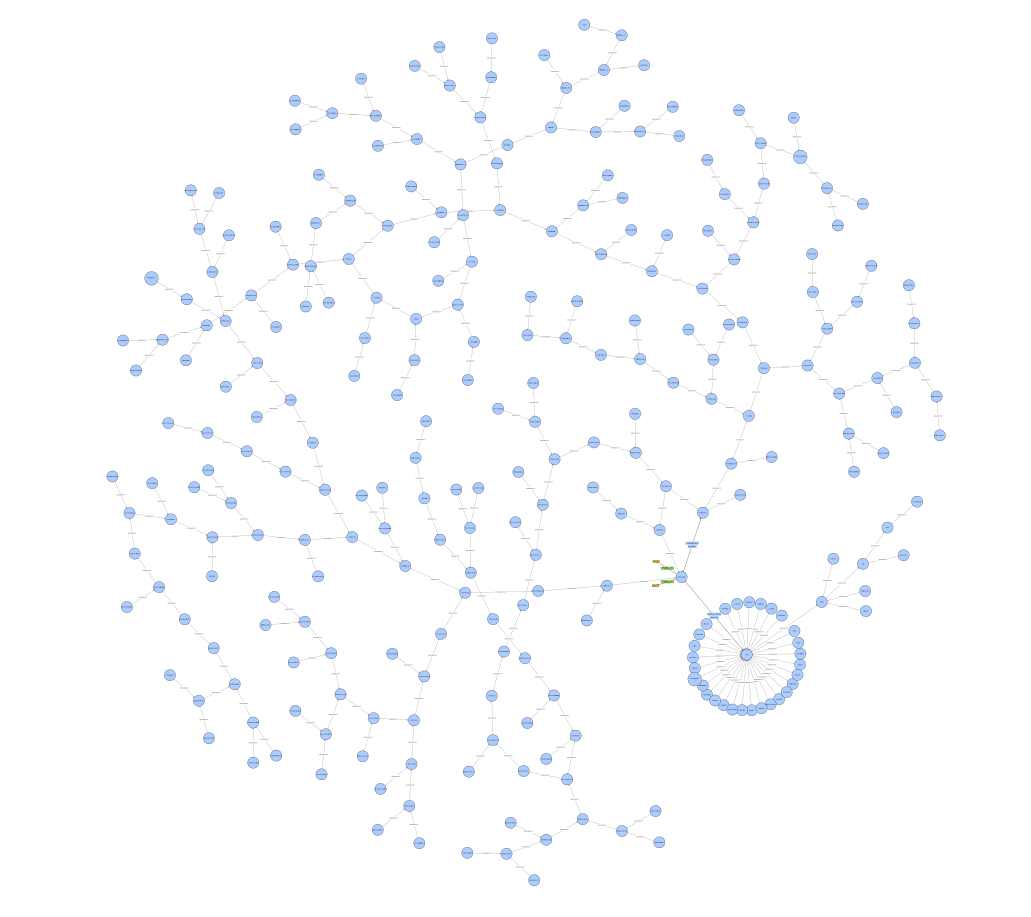
\includegraphics[width=0.8\textwidth, trim=0mm 16cm 0mm 2cm, clip]{dinosaur_onto.pdf}
	%	\caption{Онтология на разред динозаври}
	%	\label{fig:ontology_webvowl}
	%\end{figure}
	
	\newpage
	
	\section{Планиране и бъдещо развитие}\label{sec:future}
	
	\newpage
	
	\begin{thebibliography}{999}
		
		\bibitem{owlready2}
		\href{https://owlready2.readthedocs.io/en/latest/}{Owlready2}
		
		\bibitem{owl-guide}
		\href{https://www.w3.org/TR/owl-guide/}{OWL Web Ontology Language Guide}
		
		\bibitem{geol-104-dinosaurs}
		\href{https://www.geol.umd.edu/%7Etholtz/G104/lectures/104dinorise.html}{GEOL 104 Dinosaurs: A Natural History}
		
		\bibitem{ornithischia}
		\href{https://en.wikipedia.org/wiki/Ornithischia}{Ornithischia}
		
		\bibitem{thyreophora}
		\href{https://en.wikipedia.org/wiki/Thyreophora}{Thyreophora}
		
		\bibitem{cerapoda}
		\href{https://en.wikipedia.org/wiki/Cerapoda}{Cerapoda}
		
		\bibitem{saurischia}
		\href{https://en.wikipedia.org/wiki/Saurischia}{Saurischia}
		
		\bibitem{theropoda}
		\href{https://en.wikipedia.org/wiki/Theropoda}{Theropoda}
		
		\bibitem{sauropoda}
		\href{https://en.wikipedia.org/wiki/Sauropoda}{Sauropoda}
		
		
	\end{thebibliography}
	
\end{document}
